\section{Adaptive workload management through elastic scheduling}
Real time computing systems, timing constraints guaranteed are based on off line calculated parameters based on fixed parameters and worst case execution time.
But a precise estimation of tasks' computation time is tricky due to the unpredictability of low level processor mechanisms including DMA, branch prediction, cache management.
An underestimation of the resources results in critical failure, while overestimation will result in wastage of resources.
A new methodology is put forward to automatically adapt the task rates of the periodic task set with forcing programmer to provide a priori estimates of the tasks' computation time. \\
There are task scenarios, for example sensors for robotic perception that should increase the acquisition rate and hence the frequency of execution to meet a given demand.\\
Similarly, there are situations where a task may experience an overload condition and graceful degradation of the service need to be provided.\\
\textbf{\textbf{Key Idea:}} \textit{Does not rely on WCET based task budgeting, but uses a dynamic approach to tune the workload utilization.}
\begin{itemize}
	\item Kuo and Mok(1991): Load scaling technique to gracefully degrade the workload by period adjustment.
	\item Nakajima and Tezuka (1994): Using real time task to support adaptive application. Period of a task is increased whenever a deadline miss is detected for the same.
	\item Seto et al.(1997): Method for computing task period to minimize a performance index defined over task set. This approach being effective at design time to optimize a discrete control system.
	\item Lee et al.(1996): Proposes number of methods to dynamically adjust task rates in overload conditions.
	\item Becarri et al.(1999): Proposes several method to handle overload through period adjustment, but not to improve utilization in underloaded condition.
	\item Stankovic et al and Lu et.al proposed feedback mechanism to observe and adjust workload to improve utilization.
\end{itemize}

Task equated to spring with rigidity coefficient and length constraints.\\
\textbf{\textit{Note:}} \textbf{Elastic or rigidity coefficient of the task can be set inversely proportional to the importance of the task. Hence a task of lower priority is more acceptable to be shrunk to accomodate a higher priority task.}\\
\subsection*{Scope}
\begin{itemize}
	\item Main contribution is task compression algorithm. Task budgets are not known a priori and are monitored at runtime.
	\item Feedback based architecture for elastic rate adaptation. The design of this approach is similar to bandwidth sharing server implementation of Lippari et. al. 
	\item Feedback mechanism is used to measure average execution time c\textsubscript{i} and maximum execution time C\textsubscript{i}. Execution time estimate is calculated as:  Q\textsubscript{i} = c\textsubscript{i} + k(C\textsubscript{i} - c\textsubscript{i}). Execution budget is calculated as \textbf{sum of (Q\textsubscript{i}/ T\textsubscript{i})}.
	\item This value is used again by the elastic algorithm for the recalculation.
\end{itemize}
\section{Elastic task model for Adaptive Rate Control}
A novel periodic task model is proposed in which tasks periods are provided with elastic coefficients. Under this approach tasks can change there execution rate to provide different Quality of Service(QoS).
To simplify the schedulability analysis simple assumptions are taken, as is the case with RM and EDF. For which tasks with cyclic execution and fixed demand are considered.
But this assumption are too restrictive for application for which timing constraints can be more flexible and dynamic.
Works have been done to done theoretical support to such tasks using probabilistic guarantee, capacity reservation based approach or by providing an upper bound on the job chains with variable executions.
Varying tasks rate provides the possibility of handling a graceful task degradation rather than outright rejection of some tasks.
A number of approaches have been proposed for dynamic and static load balancing to handle overload conditions. In \textit{"QoS Negotiation  in  Real-Time Systems  and  Its  Applications to Automated Flight Control"} QoS is proposed as a set of negotiation options based on reward and rejection penalties.\\
This Paper tries to propose a generic way for tasks to change there execution rates and provide varying QoS under different condition.
The elastic task model works by compressing the taskset under overload condition. The compression of tasks is handled depending upon the elastic coefficient \textit{e}. Another advantage of elastic task model is when considering a new task into otherwise schedulable task set. Under a rigid task model this will not be feasible, but by using elastic task compression the new task could be accommodated.\\
The basic algorithm used to tune the elastic tasks is given below:


\begin{minipage}{\linewidth}% to keep image and caption on one page
	\makebox[\linewidth]{%        to center the image
		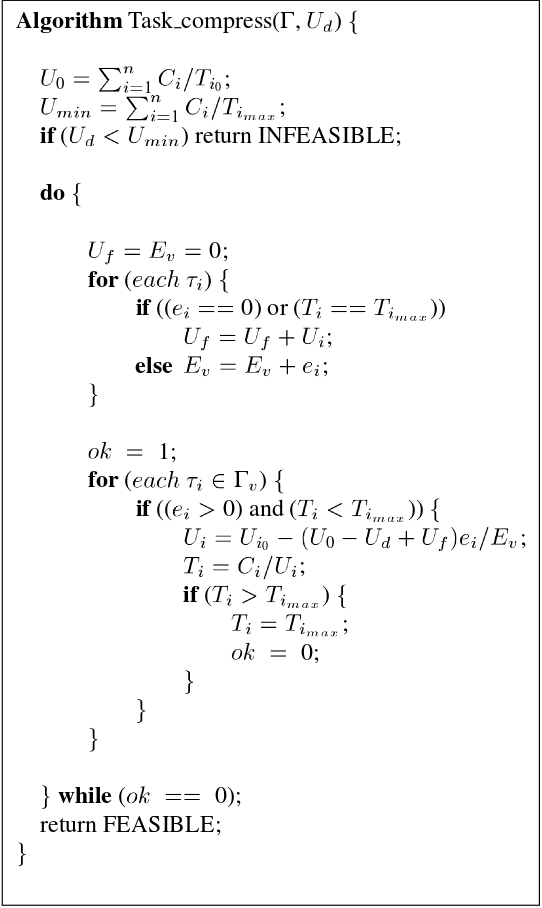
\includegraphics[scale=0.5]{Pictures/Elasic_algo.png}}
\end{minipage}

\section{Towards runtime adaptation in AUTOSAR}
This paper put forwards a method to extend the AUTOSAR mode management to implement runtime adaptation.
To realize runtime adaptation in AUTOSAR relocation of software components at runtime is required, which in turn is based on computation of adaptations during runtime.
To meet the Adaptation requirements the new model tries to meet to following challenges.
\begin{itemize}
	\item Real time requirements.
	\item Self describing components.
	\item Scheduling.
	\item ECU Independent addressing.
\end{itemize}
The runtime adaptation is implemented by two components: Adaptation Service and Adaptation Manager.
Relocating software requires control over starting and stopping of AUTOSAR Software Components, this is done by extending the system by a runtime control based on MAPE(Monitor, ANalyze, Plan and Execute) cycle.


\begin{minipage}{\linewidth}% to keep image and caption on one page
	\makebox[\linewidth]{%        to center the image
		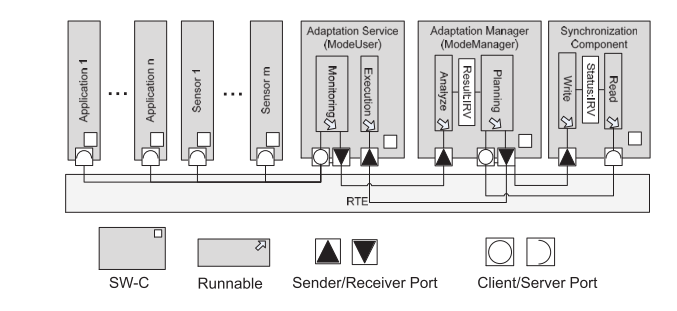
\includegraphics[scale=0.5]{Pictures/Adaptation_Manager.png}}
\end{minipage}
\begin{itemize}
	\item \textbf{Monitoring Mechanism} : Monitoring unit extends the mode manager. A request to change the mode to meet the new requirements is initiated to Mode Manager.
	\item \textbf{Analyze}: Mode manager does the analyze and planning phase. A single adaptation manager can exist in entire automotive network or to properly extend Mode manager, one Adaptation Manager shal exist per ECU. This also has the added benefit of redundancy avoiding single point of failure.
	\item \textbf{Synchronization Mechanism}: Mode Manager shall notify the Synchronization manager of the changed execution and will synchronize it across the ECUs in network.
	\item \textbf{Real-Time requirements}: The Adaptation mechanism implemented shall always be determined with respect to the component timing requirement.
	\item \textbf{Self-Describing components}: In order to check for the timing requirements the components shall publish the attributes needed for runtime verification such as end to end deadline.
	\item Scheduling: EDF Scheduling to provide better efficiency.
\end{itemize}
\section{Fast and Tight Analysis of AUTOSAR Schedule Tables.}
Proposes how to quantify the response time of the schedule table driven task set considering the offset and resource based priority threshold interference.
Two different analysis of rta and maximum time to release of a given task under a given time frame \textit{t}, as well as maximum time to completion of the given task is put forward.
First method being tight fit while the second method is an approximate estimation of the above mentioned parameters.
\section{Evaluation and Implementation of Mixed-Criticality Scheduling Approaches for Periodic Tasks}
The paper proposes a quantitative comparison of MC Approaches including: Priority assignment, Period transformation and Zero-slack scheduling.
Zero slack scheduling is improved by addressing two previously known issues: How to accommodate execution of a task after its deadline and how to handle previously unknown interferences.
% Paper on fault injection mechanisms: Authors Thorsten Piper et.al

%----------------------------------------------------------------%
%----------------------------------------------------------------%

\section{Towards the design of certifiable mixed-criticality systems.}


